\documentclass[10pt,a4paper]{article}
\usepackage[utf8]{inputenc}
\usepackage[T1]{fontenc}
\usepackage{graphicx}
\usepackage{xcolor}
\usepackage{tikz}
\usepackage{qrcode}
\usepackage{helvet}
\usepackage[margin=0mm]{geometry}
\usepackage[hidelinks]{hyperref}
\renewcommand{\familydefault}{\sfdefault}
\pagestyle{empty}
\setlength{\parindent}{0pt}

\definecolor{ClubNavy}{HTML}{09245D}
\definecolor{DeepNavy}{HTML}{03122F}
\definecolor{ElectricBlue}{HTML}{087AE8}
\definecolor{CyanAccent}{HTML}{00C8E7}
\definecolor{Ink}{HTML}{14213D}
\definecolor{Muted}{HTML}{53627A}
\definecolor{PaperBlue}{HTML}{F4F8FC}
\definecolor{LineBlue}{HTML}{DCE8F5}

\begin{document}
\begin{tikzpicture}[remember picture,overlay,shift={(current page.south west)},x=1mm,y=1mm]
  % Base and subtle technical grid.
  \fill[PaperBlue] (0,0) rectangle (210,297);
  \foreach \x in {0,10,...,210} {\draw[LineBlue,opacity=.28,line width=.15pt] (\x,0)--(\x,224);}
  \foreach \y in {0,10,...,220} {\draw[LineBlue,opacity=.28,line width=.15pt] (0,\y)--(210,\y);}

  % Cropped event artwork with the white-only club mark floating above it.
  \begin{scope}
    \clip (0,224) rectangle (210,297);
    \node[anchor=north west,inner sep=0] at (0,297)
      {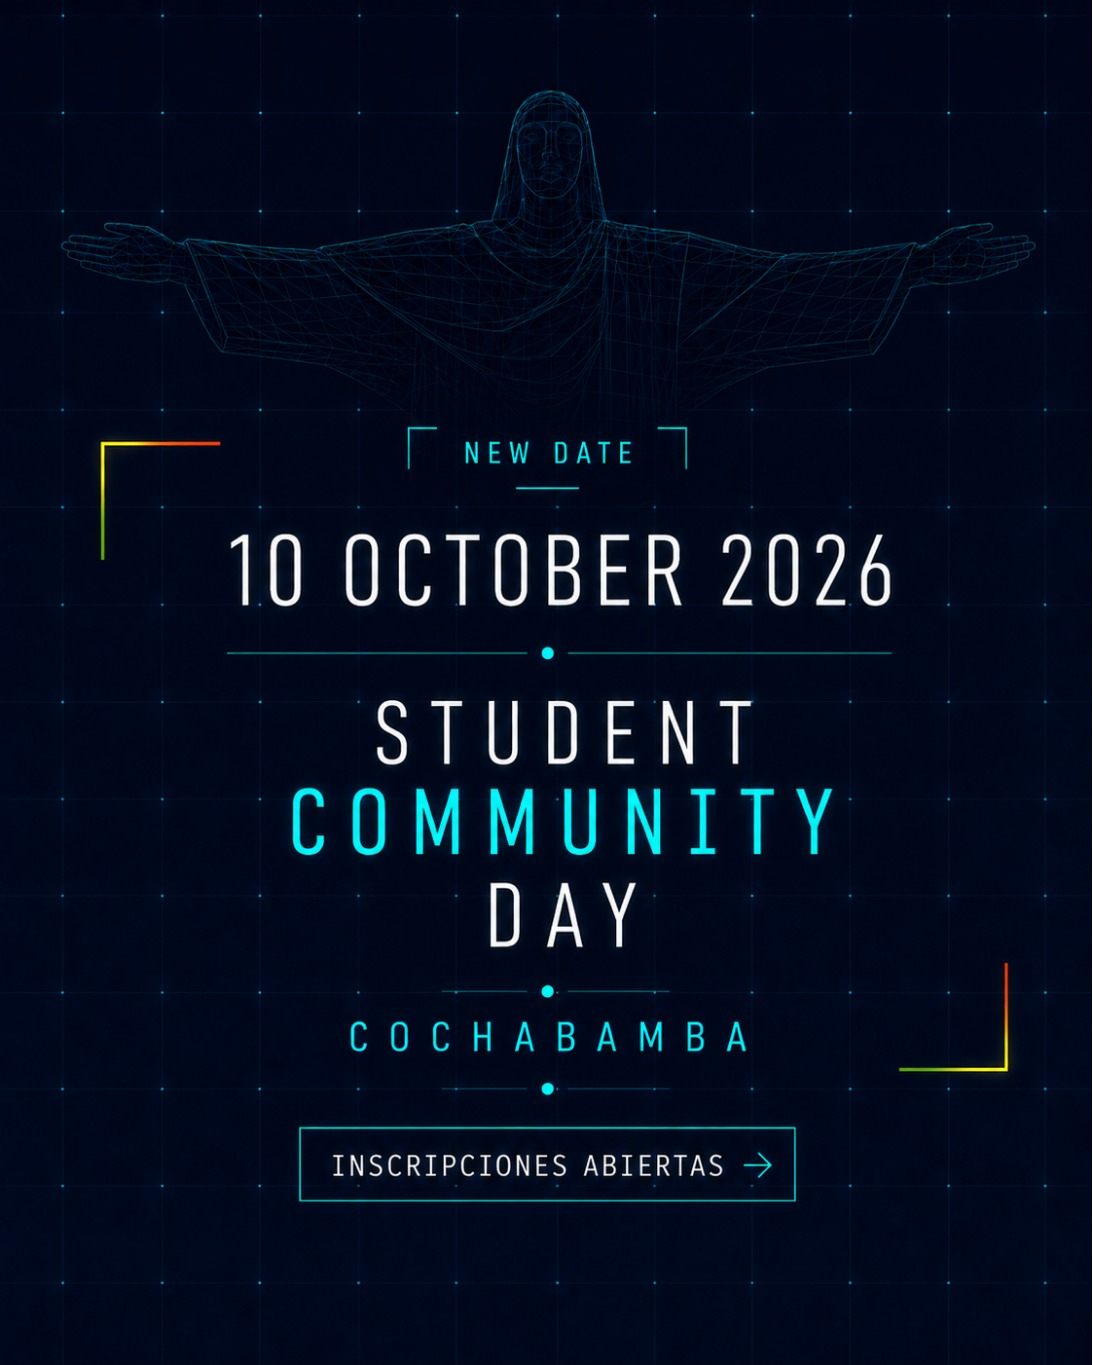
\includegraphics[width=210mm]{indice.png}};
    \fill[DeepNavy,opacity=.16] (0,224) rectangle (210,297);
    \fill[DeepNavy,opacity=.80] (0,224) rectangle (210,240);
  \end{scope}

  \node[anchor=north west,inner sep=0,opacity=.96] at (13,287)
    {
\includegraphics[width=24mm]{logo-white.png}};
  \node[anchor=north east,align=right,text=white] at (197,286)
    {\fontsize{8}{9}\selectfont\bfseries AWS STUDENT BUILDER GROUP\\[-1pt]
     \fontsize{7}{8}\selectfont\mdseries UPB COCHABAMBA};
  \draw[CyanAccent,line width=1.2pt] (149,274)--(197,274);
  \node[anchor=south west,text=white] at (13,228)
    {\fontsize{8}{9}\selectfont\bfseries \DocumentType};

  % Recipient block.
  \node[anchor=north west,text=ElectricBlue] at (18,214)
    {\fontsize{7.5}{9}\selectfont\bfseries \RecipientEyebrow};
  \node[anchor=north west,text width=174mm,text=Ink] at (18,207)
    {\fontsize{15}{17}\selectfont\bfseries \RecipientName};
  \node[anchor=north west,text width=174mm,text=Muted] at (18,197)
    {\fontsize{9}{11}\selectfont \RecipientRole};
  \draw[ElectricBlue,line width=.8pt] (18,188)--(52,188);

  % Main message.
  \node[anchor=north west,text width=174mm,align=justify,text=Ink] at (18,181)
    {\fontsize{10}{14}\selectfont
     \Opening

     \vspace{3mm}
     El \textbf{AWS Student Builder Group UPB Cbba} tiene el agrado de invitarle al
     \textbf{AWS Student Community Day (SCD) Bolivia 2026}, una jornada creada
     para reunir a estudiantes interesados en tecnología y computación en la nube.

     \vspace{2.5mm}
     Durante la jornada, los asistentes podrán ampliar su perspectiva sobre el
     ecosistema tecnológico, descubrir nuevas posibilidades de la nube y conectar
     con estudiantes que comparten el interés por aprender, crear y transformar
     ideas en proyectos. Nos encantaría contar con la participación de su institución.};

  % Event information card.
  \fill[white,rounded corners=2mm] (18,77) rectangle (192,118);
  \draw[LineBlue,rounded corners=2mm,line width=.7pt] (18,77) rectangle (192,118);
  \fill[ElectricBlue,rounded corners=2mm] (18,77) rectangle (22,118);
  \node[anchor=north west,text=Ink] at (29,110)
    {\fontsize{8}{9}\selectfont\bfseries SÁBADO};
  \node[anchor=north west,text=ClubNavy] at (29,102)
    {\fontsize{19}{20}\selectfont\bfseries 10 OCT};
  \node[anchor=north west,text=Muted] at (29,88)
    {\fontsize{8}{9}\selectfont 2026};

  \draw[LineBlue,line width=.7pt] (70,84)--(70,111);
  \node[anchor=north west,text=ElectricBlue] at (79,109)
    {\fontsize{7}{8}\selectfont\bfseries HORARIO};
  \node[anchor=north west,text=Ink] at (79,101)
    {\fontsize{11}{12}\selectfont\bfseries 09:00 -- 17:30};
  \node[anchor=north west,text=ElectricBlue] at (79,91)
    {\fontsize{7}{8}\selectfont\bfseries LUGAR};
  \node[anchor=north west,text width=70mm,text=Ink] at (79,87)
    {\fontsize{7.5}{8.7}\selectfont UPB Cochabamba\\Campus Julio León Prado};

  \node[anchor=center,inner sep=0] at (175,97.5)
    {\qrcode[height=25mm,level=M]{https://luma.com/r65j1ukn}};
  \node[anchor=north,text=Muted] at (175,83)
    {\fontsize{5.8}{7}\selectfont ESCANEA PARA REGISTRARTE};

  % Closing and organizing signature.
  \node[anchor=north west,text width=112mm,text=Ink] at (18,67)
    {\fontsize{9}{12}\selectfont
     Agradecemos su atención y esperamos darle la bienvenida en esta jornada.

     \vspace{4mm}
     \textbf{Atentamente,}\\[2mm]
     \textbf{AWS Student Builder Group UPB Cbba}\\[-1mm]
     \textcolor{Muted}{Comité organizador}\\[1mm]
     \href{mailto:sbgcbba@upb.edu}{\textcolor{ElectricBlue}{sbgcbba@upb.edu}}};

  \fill[ClubNavy,rounded corners=1.5mm] (143,34) rectangle (192,65);
  \node[anchor=north,text=CyanAccent] at (167.5,59)
    {\fontsize{6.5}{8}\selectfont\bfseries INSCRIPCIONES ABIERTAS};
  \node[anchor=north,text=white] at (167.5,51)
    {\href{https://luma.com/r65j1ukn}{\fontsize{8.5}{10}\selectfont\bfseries luma.com/r65j1ukn}};

  % Footer.
  \fill[ClubNavy] (0,0) rectangle (210,20);
  \fill[CyanAccent] (0,20) rectangle (210,21.5);
  \node[anchor=west,text=white] at (18,10)
    {\fontsize{7}{8}\selectfont 10 DE OCTUBRE DE 2026 \quad\textcolor{CyanAccent}{\textbullet}\quad COCHABAMBA};
  \node[anchor=east,text=white] at (192,10)
    {\fontsize{7}{8}\selectfont\bfseries STUDENT COMMUNITY DAY};
\end{tikzpicture}
\null
\end{document}
